% This is a LaTeX template kindly taken from Jernej Debevec.
% Provided by Miha Muskinja for the purpose of the seminar I in the 1st year
% of the 2nd cycle of the study of physics at the Faculty of Mathematics and Physics, University of Ljubljana.
% I have edited it to suit my needs.

% Set the document class and options
\documentclass[10pt, titlepage, a4paper]{article}
\usepackage[a4paper, inner=2.5cm, outer=2.5cm, top=2.25cm, bottom=2.25cm]{geometry}
\usepackage{graphicx}
\usepackage{hyperref}
\usepackage{wrapfig}
\usepackage{bm}
\usepackage{amsmath}
\usepackage{amssymb}
\usepackage{float}
\usepackage{accents}
\usepackage{cleveref}
\usepackage{subcaption}
\hypersetup{colorlinks=true}
\setlength{\parindent}{0pt}

\usepackage[
    backend=biber,
    style=numeric,
    natbib=true,
    sorting=none,
    url=false, 
    doi=true,
    eprint=false
]{biblatex}
\addbibresource{mod204.bib}
\DeclareFieldFormat{doi}{%
    \textsc{doi}\addcolon\space
    \href{https://doi.org/#1}{\textcolor{red}{\nolinkurl{#1}}}%
}

\usepackage{tikz}
\usetikzlibrary{positioning,arrows}
\usetikzlibrary{arrows.meta}
\usetikzlibrary{decorations.pathmorphing}
\usetikzlibrary{decorations.markings}
\tikzset{>=Stealth}

% Prototype colors from cmr.tropical
\definecolor{color1}{RGB}{144,14,165}
\definecolor{color2}{RGB}{168,8,146}
\definecolor{color3}{RGB}{188,7,122}
\definecolor{color4}{RGB}{205,27,92}
\definecolor{color5}{RGB}{215,53,64}
\definecolor{color6}{RGB}{217,81,40}
\definecolor{color7}{RGB}{214,107,19}
\definecolor{color8}{RGB}{206,132,3}
\definecolor{color9}{RGB}{192,156,16}
\definecolor{color10}{RGB}{169,180,47}
\definecolor{color11}{RGB}{139,201,81}
\definecolor{color12}{RGB}{94,221,125}

% Some macros for commonly used symbols in physics/quantum mechanics
\newcommand{\bb}[1]{\bm#1}
\newcommand{\dd}{\mathrm{d}}
\newcommand{\pp}{\partial}
\newcommand{\dg}{\dagger}
\newcommand{\la}{\langle}
\newcommand{\ra}{\rangle}
\newcommand{\id}{\mathbb{1}}
\newcommand{\T}{\mathsf{T}}
\newcommand{\ua}{\uparrow\>}
\newcommand{\da}{\downarrow\>}
\newcommand{\mc}[1]{\mathcal{#1}}
\newcommand\thickbar[1]{\accentset{\rule{.5em}{.03em}}{#1}}
\renewcommand{\bar}{\thickbar}

% Code highlighting
\usepackage{minted}
\usepackage{listings}
\usepackage{tcolorbox}
\usepackage[export]{adjustbox}
\tcbuselibrary{listings, minted, skins, breakable}

\newtcblisting{pythonlst}{listing only, minted language=python3, minted style=paraiso-dark,
    colback=bg, enhanced jigsaw, frame hidden, breakable=true, minted options={, 
    fontsize=\footnotesize, tabsize=2, breaklines, autogobble}}

\setminted[python3]{bgcolor=bg, fontsize=\footnotesize}
\definecolor{inline}{RGB}{187,57,82}
\definecolor{bg}{RGB}{40,40,40}


% Start the document
\begin{document}

% The title page
\begin{titlepage}
{\centering

\includegraphics[width=6cm]{logo_fmf.pdf}

\vspace{0.8cm}
{\small Department of Physics}

\vspace{5cm}
\vspace{0.5cm}
{\huge\textbf{Successive Over-Relaxation for Boundary Value Problems}} \\
\vspace{0.5cm}
{\large\textbf{5. Assignment for Model Analysis 2, 2025/26}}

\vfill
\textbf{Author:} Marko Urbanč (28232019) \\
\textbf{Professor:} Prof. dr. Simon Širca  \\ 
\textbf{Advisor:}  doc. dr. Miha Mihovilovič \\


\vspace{1cm}
Ljubljana, March 2026 \\
}

\vspace{3cm}
\end{titlepage}

% Add table of contents
\hypersetup{pageanchor=true}
\pagenumbering{roman}
\setcounter{page}{2}
\tableofcontents
\vspace{1cm}

% Proceed with the main body
\pagenumbering{arabic}

% Sections based on typical Model Analysis structure
\section{Introduction}
This week we finally move on from shooting methods to a more general class of methods for solving boundary value problems: relaxation methods. Specifically we will be taking 
a look at the Successive Over-Relaxation (SOR) method, which is an iterative method for solving linear systems of equations that arise from discretizing partial differential equations (PDEs). 
The SOR method is an extension of the Gauss-Seidel method, which itself is an improvement over the Jacobi method. The key idea behind SOR is to introduce a relaxation factor that can accelerate the convergence of the iterative process.
That is to say, that instead of simply using the new values computed in the current iteration, we intentionally "over-relax" the update by a factor $\omega$ (the relaxation factor), which can be tuned to achieve faster convergence. \\

The relaxation factor $\omega$ in bounded between 0 and 2, where $\omega = 1$ corresponds to the Gauss-Seidel method, $\omega < 1$ corresponds to under-relaxation, and $\omega > 1$ corresponds to over-relaxation. $\omega=2$ 
corresponds to the limit of stability, and values of $\omega \geq 2$ will lead to divergence. The optimal choice of $\omega$ depends on the specific problem being solved, and finding it can 
significantly reduce the number of iterations required for convergence. Specifically, $\omega$ depends on the spectral radius of the iteration matrix $\rho_\text{jac}$ as:

\begin{equation}
    \omega = \frac{2}{1 + \sqrt{1 - \rho_\text{jac}^2}}\>.
    \label{eq:omega-rho}
\end{equation}

The optimal $\omega$ for a full square grid can be approximated as:

\begin{equation}
    \omega_\text{opt} \approx \frac{2}{1 + \frac{\pi}{N}}\>,
    \label{eq:omega-opt}
\end{equation}

where $N$ is the number of grid points in one dimension. In our assignment we will use the following ansatz for the relaxation factor:

\begin{equation}
    \omega = \frac{2}{1 + \alpha \frac{\pi}{N}}\>,
    \label{eq:omega-alpha}
\end{equation}

where $\alpha$ is a tunable parameter that we will need to optimize for our specific problem. \\

Since the SOR method iterative process is symmetric with respect to grid point parity, we can perform updates in a checkerboard pattern in two half-steps. This allows us to 
use an even faster approach for convergence called \textbf{Chebyshev Acceleration}, which is a technique that optimizes the relaxation factor $\omega$ over the course of half-iteration steps
as: 

\begin{flalign}
    \omega^(0) &= 1 \>, \\
    \omega^{(1/2)} &= \frac{1}{1 - \frac{1}{2}\rho^2_\text{jac}} \>, \\
    \omega^{(n) + 1/2} &= \frac{1}{1 - \frac{1}{4}\omega^{(n)}\rho^2_\text{jac}} \>. 
\end{flalign}

This approach allows us to achieve convergence in a number of iterations that scales as $\mathcal{O}(N)$, which is a significant improvement 
over the $\mathcal{O}(N^2)$ scaling of the standard SOR method. For this to work however we need to have a good estimate of the spectral radius $\rho_\text{jac}$, which we 
can obtain by tuning $\alpha$ in \Cref{eq:omega-alpha} and using the optimal $\omega$ in \Cref{eq:omega-rho} to get $\rho_\text{jac}$.

\section{Task}
\subsection{Steady-State Velocity Profile and Poisseuille Coefficient}
Using the SOR method, we will solve the Poisson equation for the velocity profile of a fluid flowing through a pipe with a \textit{'house-like'} cross-section. We are instructed to 
pay close attention to the correct treatment of cases where the boundary conditions are not defined at the grid points, but are instead defined at the midpoints between grid points. 
We need to find the optimal parameter $\alpha$ for the relaxation factor $\omega$ and test out the Chebyshev acceleration method. Finally, we need to 
compute the Poisseuille coefficient for the flow.

\begin{figure}[H]
    \centering
    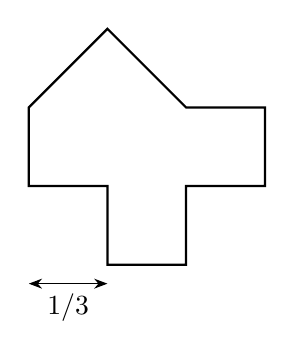
\begin{tikzpicture}[scale=3]
        % Let s = 1/3
        \def\s{0.333}
        
        % Draw the pipe cross-section outline
        \draw[thick] 
            % Start bottom left of stem
            (\s, 0)
            -- (\s, \s)          % up left side of stem
            -- (0, \s)           % left to left edge
            -- (0, 2*\s)         % up left body
            % Roof left diagonal: from (0, 2s) to (1.5s, 3s) i.e. peak
            -- (1.0*\s, 3*\s)    % up to roof peak
            -- (2*\s, 2*\s)        % down to right notch top  
            -- (1, 2*\s)         % right across
            -- (1, \s)           % down right body
            -- (2*\s, \s)        % left to right of stem
            -- (2*\s, 0)         % down right side of stem
            -- cycle;            % back to start
        
        % 1/3 dimension arrow
        \draw[<->] (0, -0.08) -- (\s, -0.08) node[midway, below] {$1/3$};
    \end{tikzpicture}
\end{figure}

\subsection{Steady-State Temperature Distribution in a Cylinder}
Next, we will solve the steady-state heat equation in an equilateral cylindrical geometry with a constant heat flux at the bottom of the cylinder. The cylindrical surface is 
cut horizontally in half, with each half at a different temperature. The top surface of the cylinder is kept at the same temperature as the lower half of the cylinder. 
Our goal is to find the steady-state temperature distribution. We need to then repeat this calculation for the same geometry, but where the upper half of the cylinder is thermally insulated.

\begin{figure}[H]
    \centering
    \begin{subfigure}{0.48\textwidth}
        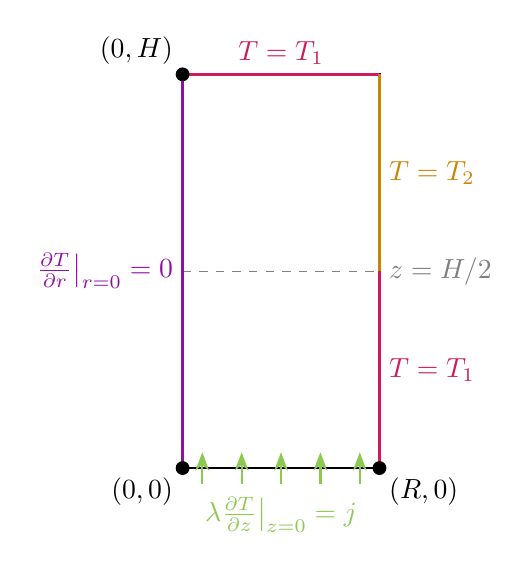
\begin{tikzpicture}[scale=2.5]
            % Draw domain rectangle
            \draw[thick] (0,0) rectangle (1,2);
            
            \draw[dashed, gray] (0,1) -- (1,1);
                
            \foreach \x in {0.1, 0.3, 0.5, 0.7, 0.9} {
                \draw[->, thick, color11] (\x, -0.08) -- (\x, 0.08);
            }
            \node[below, color11] at (0.5, -0.1) {$\lambda \frac{\partial T}{\partial z}\big|_{z=0} = j$};
            
            \draw[color4, very thick] (0,2) -- (1,2);
            \node[above, color4] at (0.5, 2) {$T = T_1$};
            
            \draw[color1, very thick] (0,0) -- (0,2);
            \node[left, color1] at (0, 1) {$\frac{\partial T}{\partial r}\big|_{r=0} = 0$};
            
            \draw[color4, very thick] (1,0) -- (1,1);
            \node[right, color4] at (1, 0.5) {$T = T_1$};
            
            \draw[color8, very thick] (1,1) -- (1,2);
            \node[right, color8] at (1, 1.5) {$T = T_2$};
            
            % Split label
            \node[right, gray] at (1, 1) {$z = H/2$};
        
            % Corner coordinates
            \node[below left] at (0,0) {$(0,0)$};
            \node[above left] at (0,2) {$(0,H)$};
            \node[below right] at (1,0) {$(R,0)$};
            \fill[black] (0, 0) circle (1.0pt);
            \fill[black] (0, 2) circle (1.0pt);
            \fill[black] (1, 0) circle (1.0pt);
            
        \end{tikzpicture}
        \caption{Case 1: \textbf{Dirichlet} boundary condition at the upper half of the cylinder.}
        \label{fig:case1}
    \end{subfigure}
    \hfill
    \begin{subfigure}{0.48\textwidth}
        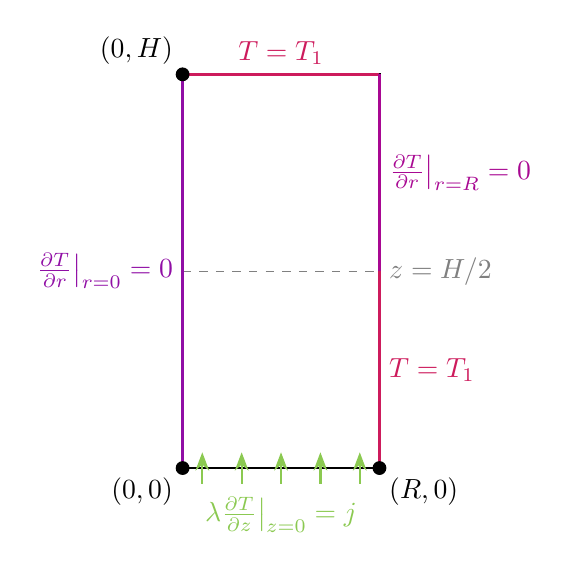
\begin{tikzpicture}[scale=2.5]
            % Draw domain rectangle
            \draw[thick] (0,0) rectangle (1,2);
            
            \draw[dashed, gray] (0,1) -- (1,1);
                
            \foreach \x in {0.1, 0.3, 0.5, 0.7, 0.9} {
                \draw[->, thick, color11] (\x, -0.08) -- (\x, 0.08);
            }
            \node[below, color11] at (0.5, -0.1) {$\lambda \frac{\partial T}{\partial z}\big|_{z=0} = j$};
            
            \draw[color4, very thick] (0,2) -- (1,2);
            \node[above, color4] at (0.5, 2) {$T = T_1$};
            
            \draw[color1, very thick] (0,0) -- (0,2);
            \node[left, color1] at (0, 1) {$\frac{\partial T}{\partial r}\big|_{r=0} = 0$};
            
            \draw[color4, very thick] (1,0) -- (1,1);
            \node[right, color4] at (1, 0.5) {$T = T_1$};
            
            \draw[color2, very thick] (1,1) -- (1,2);
            \node[right, color2] at (1, 1.5) {$\frac{\partial T}{\partial r}\big|_{r=R} = 0$};
            
            % Split label
            \node[right, gray] at (1, 1) {$z = H/2$};
        
            % Corner coordinates
            \node[below left] at (0,0) {$(0,0)$};
            \node[above left] at (0,2) {$(0,H)$};
            \node[below right] at (1,0) {$(R,0)$};
            \fill[black] (0, 0) circle (1.0pt);
            \fill[black] (0, 2) circle (1.0pt);
            \fill[black] (1, 0) circle (1.0pt);
            
        \end{tikzpicture}
        \caption{Case 2: \textbf{Neumann} boundary condition at the upper half of the cylinder.}
        \label{fig:case2}
    \end{subfigure}
\end{figure}


\section{Solution Overview}
\section{Results}
\section{Conclusion and Comments}

% Add references
% \newpage
% \bibliographystyle{unsrt}
% \bibliography{main}

% End document
\end{document}
